\newpage


\section{Moderne Cyberbedrohungen}\label{sec:moderne-cyberbedrohungen}
\todo[inline]{Eventuell Einleitungstext schreiben}

\subsection{Trends und Entwicklungen in der Cyberkriminalität}\label{subsec:trends-und-entwicklungen-in-der-cyberkriminalitat}
In den letzten Jahren hat die Anzahl der Cyberkriminalitätsfälle in Deutschland stark zugenommen.
So wurden zwar für das Jahr 2022 ein Rückgang von ungefähr 6.5\% gegenüber dem Vorjahr an erfassten Fällen aufgezeichnet, jedoch bildet sich in dem Zeitraum von 2012 bis 2022 ein Gesamtwachstum von ungefähr 112\% an erfassten Cyberkriminalitätsfällen\autocite[\vglf][]{bka-cyberkriminalitaet}.

Analog zu der Anzahl der aufgezeichneten Fälle steigen auch die Kosten, die Cyberkriminalität verursacht, sowie die Ausgaben die für IT-Sicherheit in Deutschland vorgenommen werden stetig.
2018 haben Cyberkriminalitätsvorfälle deutschen Unternehmen durchschnittlich 13,12 Millionen US-Dollar\footnote{Heutiger Wert ungefähr 10,23 Millionen Euro} gekostet, was gegenüber dem Vorjahr ein Zuwachs von ungefähr 18\% darstellt\autocite[\vglf][]{accenture-cyberkrime-kosten}.
2021 wurden so ungefähr 6,9 Milliarden Euro für IT-Sicherheitsmaßnahmen ausgegeben, was einem Zuwachs von ungefähr 22\% gegenüber dem Vorjahr entspricht\autocite[\vglf][]{bitkom-itsicherheit}, davon wurden geschätzt 1,7 Milliarden Euro für Softwarelösungen ausgegeben\autocite[\vglf][]{bitkom-itsicherheit-segment}.

\subsection[Arten von Cyberbedrohungen]{Arten von Cyberbedrohungen - Malware, Phishing, DDos}\label{subsec:arten-von-cyberbedrohungen---malware-phishing-ddos}
Wie die Kosten und Ausgaben für Cyberkriminalität steigen auch die möglichen Methoden der Angreifer.
\autoref{fig:cybercrime-chart-absolute} zeigt, dass die Anzahl der aufgezeichneten Fälle von Cyberkriminalität fast stetig zunimmt.

\begin{figure}[htpb]
    \centering
    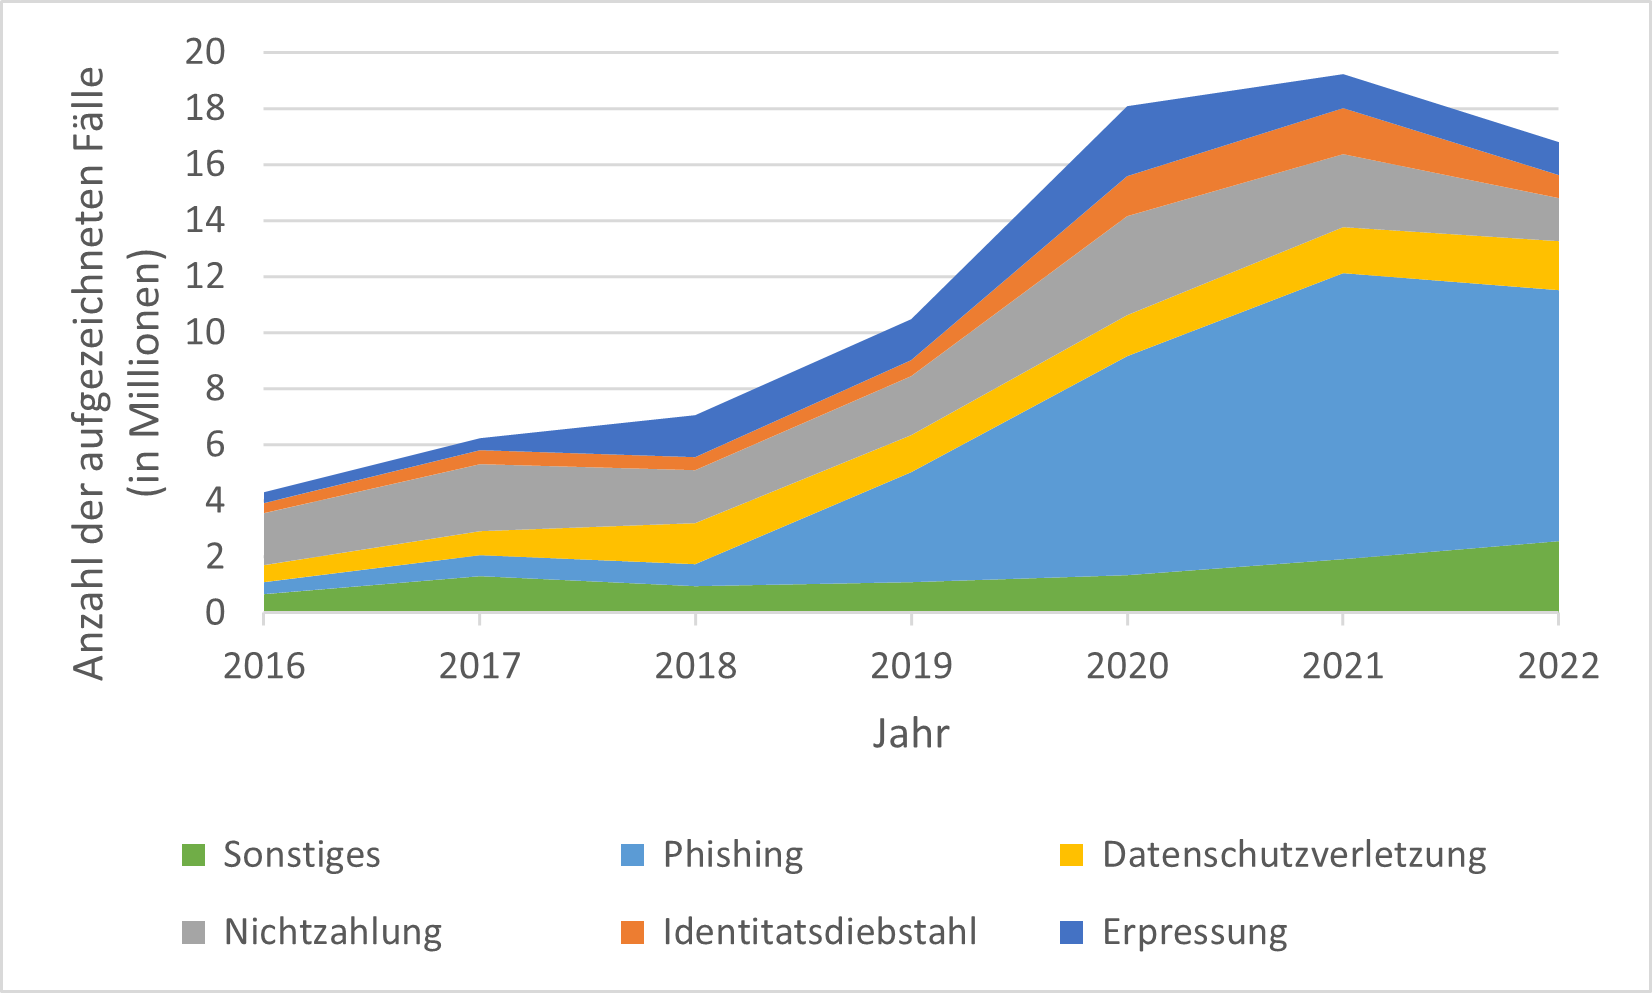
\includegraphics[width = 0.75\linewidth]{src/abbildungen/Aufgezeichnete_Cyberkriminalitaet}
    \caption[Erfasste Fälle von Cyberkriminalität nach Typ]{Erfasste Fälle von Cyberkriminalität nach Typ\footnotemark\newline Stand September 2023}
    \label{fig:cybercrime-chart-absolute}
\end{figure}\ \footnotetext{\cite[\vglf][]{statista-cybersecurity-cybercrime}}
\todo[inline]{Eventuell Float entfernen, um Fußnote anzupassen!}
Besonders der Anteil, der Phishingangriffe hat im Vergleich zu 2018 stark zugenommen, wie \autoref{fig:cybercrime-chart-relative} darstellt.
\begin{figure}[htpb]
    \centering
    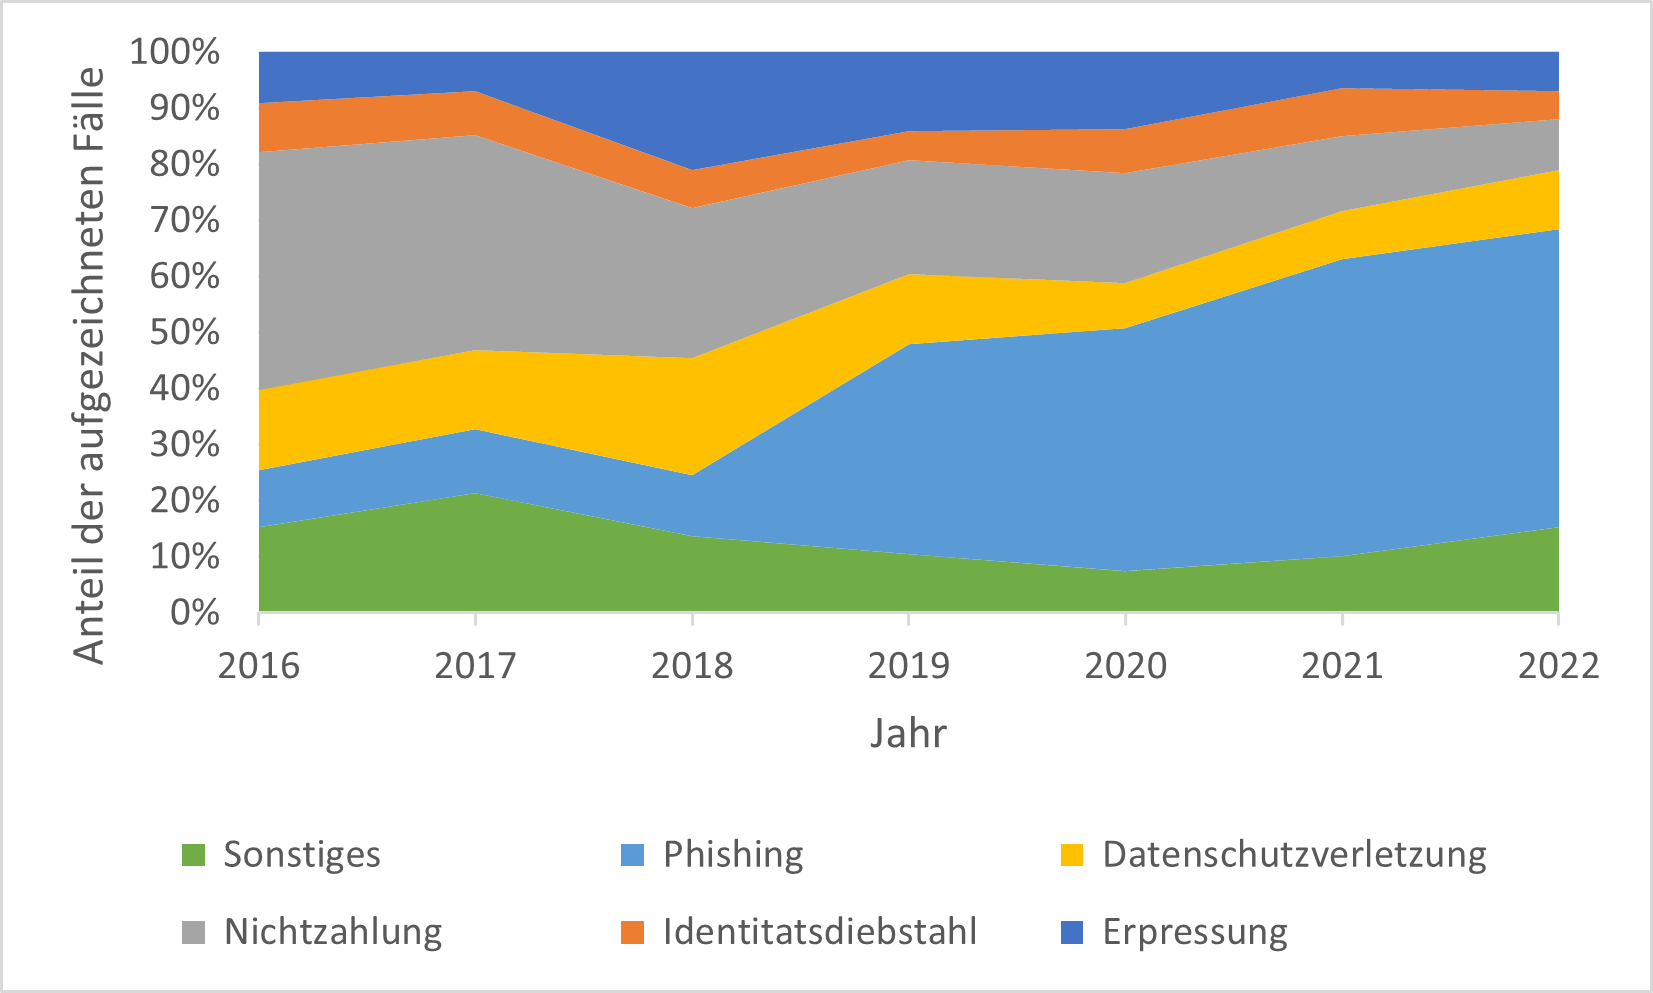
\includegraphics[width = 0.75\linewidth]{src/abbildungen/Anteile_Cyberkriminalitaet}
    \caption[Anteil einzelner Cyberkriminalitätstypen]{Anteil einzelner Cyberkriminalitätstypen\footnotemark\newline Stand September 2023}
    \label{fig:cybercrime-chart-relative}
\end{figure}\ \footnotetext{\cite[\vglf][]{statista-cybersecurity-cybercrime}}

